\paragraph{Cell line development with CHO cells}
Cell line development (CLD) is a process of generating single cell-derived clones that produce high and consistent levels of target therapeutic protein [TODO cite pharma.lonza.com/offerings/mammalian/cell-line-development]. Therapeutic proteins in this case are so-called recombinant proteins and they are spreadly used in the biomedical research, medicine production and for many different therapeutic needs like, for example, vaccines or monoclonal antibodies (mAbs) [TODO cite Ohtake 2013, Jefferis 2021, Funaro 1996]. A recombinant protein is defined by [cite Barbeau, J] as a modified or manipulated protein encoded by a recombinant DNA. Recombinant DNA in its turn consists of a plasmid, where the genes of a target protein of interest are cloned downstream of a promoter region. As soon as this plasmid will be transfected to a host cell (for example some mammalian cells that are able to produce the protein), the host wil start to express of this protein of interest. In nowadays industry and research there is a great need for production of recombinant proteins in high volumetric amounts and of a good quality [TODO cite Tihanyi 2020]. That is why the goal on many researches is in recombinant protein production is to create a their efficient expression and high-throughput systems to improve the CLD processes [cite Tihanyi 2020].


One of the most popular host cells used in CLD and in this work specifically are chinese hamster ovary (CHO) cells [cite Castan 2018]. Altough different cells can be used as hosts like bacterial, plant-based, yeast cells, the most popular ones remain mammalian [cite Beckman]. The reason behind this popularity hides in the fact that they can produce diverse correctly folded proteins and most importantly they have high productivity protein production rates. Productivity rate is measured in titre of produced protein, and CHO cells can reach 0.1 - 1 g/L in batch and 1-10 g/L in fed-batch cultures [cite Tihanyi 2020]. Mostly all of the mAbs are produced using CHO cells [cite Lalonde 2017]. Companies mostly use the same host cell line for their productions because already checked and qualified cells simplify the road to the clinic [cite Tihanyi 2020]. That is why current research has a wide applicability.

However there is a downside in using CHO as host cells - they are well-known by their instability. As a rapidly growing immortal cells CHO also genomically unstable and extremely heterogeous which ususally leads to their main problem - production instability. The problem of choosing the stable and high producing clones that simutaneously will be able to express protein quailitatively and quantitably over time is essentially the main goal of nowadays research. The big challenge in manufacturing here are the time and costs of production. Currently a lot of research attention is dedicated to the reduction of both as well as to developing techniques of high-throughput clone screening and characterization [cite Tihanyi 2020]. The latter one is of interest for this thesis. With the great amounts of data acquired over time and the development of the computational modelling and statistical analysis it is possible now to do the analysis \textit{in silico}, meaning - computationally without intervening into the cells instead of the usual \textit{in vitro} analysis.

\paragraph{CLD steps}
\begin{figure}[H]
	\begin{center}
		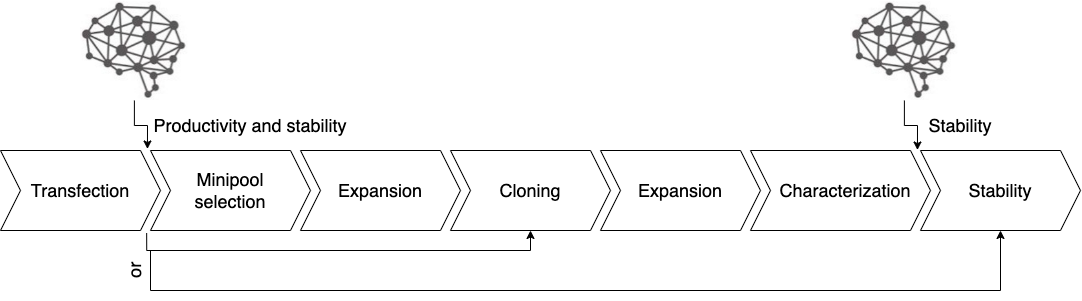
\includegraphics[width=0.8\linewidth]{bilder/CLD.png}
		\caption{CLD process steps}\label{fig:cls-steps}
	\end{center}
\end{figure}

First step of CLD is called transfection - the introduction of the gene of interest (GOI or a DNA vector or alternatively an expression vector) to CHO cells. And it has two main problems: first is that the transfection mostly results in a vector being inserted into a random site within a host cell genome and second, that it generally has low efficiency of integration [cite Tihanyi]. It is important to transfect a GOI into an optimal site of genome to secure a high protein expression over time during protein production, however pratically transfection happens into a random location of genome. In cases when the gene was transfected into the inactive site of genome (and essentially the majority of genome is transriptionally inactive) the cell will likely not be able to express the gene [cite Castan, Hong 2018].

The second step of the process is selection of cells minipools that have successful and stable gene integrations for further expansion and cloning. The reason why not all of them are suitable is the following: during the transfection step only 80\% of the cells will recieve a vector of GOI [cite Castan]. Only a small percent of these cells actually integrate a vector into the genome and, as mentioned above, only a fraction of those are able to stabily express the protein. [a better reference needed Shin 2020]. After the best mini pools are selected, they will be expanded.

The third step in CLD is to clone the cells. Chosen stable pools of cells are phenotypically and genetically diverse - meaning they have different growth rates, metabolic profile and etc. This is not ideal for industrial production - all the cells used for protein production should be derived from the same clone [cite [25] from Castan]. 

Once the cells are cloned, phenotypical and genetical heterogeneity is reduced, the next step is to charaterize the cells for their expression of the GOI. One has to estimate clones productivity and stability. Such observations may take up to 90 days (usually the checks are made on the day 30, day 60 and day 90). If the clones remain stable after this time and are able to express enough of the protein, then they are suitable for further production. However this last step consumes a lot of time and maintaining costs for feeding and analysing the cells.Predicting productivity and stability of the cells on ealier stages would reduce this time significantly or even allow to escape this process completely. 